\msection{\Wasm}
\label{sota:wasm}

%% For the intro
 % In 2014, Alon Zakai and colleagues proposed Emscripten \cite{emscripten}. 
% Emscripten used a strict subset of JavaScript, asm.js, to allow low-level code such as C to be compiled to JavaScript. 
% Asm.js was faster than JavaScript because it limited the language features to those that can be optimized in the LLVM pipeline. 
% Notably, Asm.js demonstrated that client-code could be improved with the right language design and standardization.
% Wasm marked the breaking point of several failed attempts of porting code but JavaScript to the web browser \cite{javaapplet,activex,silverlight}.
% Previous alternatives largely failed to gain traction, primarily due to security concerns and a lack of consensus among browser vendors.
% The announcement of \wasm\ marked the first step into the standardization of bytecode in the web environment. 

% History
The W3C publicly announced the \Wasm language in 2017 as the four scripting language supported in all major web browser vendors.
\wasm\ is a binary instruction format for a stack-based virtual machine and was officially consolidated by the work of Haas \etal \cite{Haas_2017} in 2017. 
Wasm is designed to be fast, portable, self-contained and secure, and it promises to outperform JavaScript execution \cite{Haas_2017}. 

% Current state
Since 2017, the adoption of \wasm\ keeps growing. 
For example; Adobe, announced a full online version of Photoshop\footnote{\url{https://twitter.com/Adobe/status/1453034805004685313?s=20&t=Zf1N7-WmzecA0K4V8R69lw}} written in WebAssembly;  game companies moved their development from JavaScript to Wasm like is the case of a full Minecraft version\footnote{\url{https://satoshinm.github.io/NetCraft/}}. 
Moreover, WebAssembly has been evolving outside web browsers since its first announcement.
Some works demonstrated that using WebAssembly as an intermediate layer is better in terms of startup and memory usage than containerization and virtualization \cite{pMendkiServerless, 1244493Jacobsson}. 
Consequently, in 2019, the Bytecode Alliance \cite{bytecodealliance} proposed WebAssembly System Interface (WASI) \cite{WASI}. 
WASI pioneered the execution of \wasm\ with a POSIX system interface protocol, making possible to execute Wasm directly in the operating system. 
Therefore, it standardizes the adoption of \wasm\ in heterogeneous platforms \cite{bryant2020webassembly}, making it suitable standalone and backend execution scenarios \cite{9640153, wen2020wasmachine}.

% How to generate
%\msubsection{\Wasm's generation and binary format}
%\todo{Replace by Rust example}
%\todo{Annotate the Wasm code with the sections offset and length}
%\todo{Instantiate each one of the previously mentioned concepts}
%\todo{Improve some metadata, size of the code, etc}
%\todo{FIX: linerefs}

\msubsection{\Wasm's generation}

\Wasm programs are pre-compiled from source languages like C/C++, Rust, or Go, which means that it can benefit from the optimizations of the source language compiler.
The resulting \wasm program is like a traditional shared library, containing instruction codes, symbols, and exported functions. 
A host environment is in charge of complementing the Wasm program, such as providing external functions required for execution within the host engine. 
For instance, functions for interacting with an HTML page's DOM are imported into the Wasm binary when invoked from JavaScript code. 

\begin{minipage}{0.9\textwidth}
    
    \begin{minipage}[b]{1.0\linewidth}
        \lstset{language=C,caption={Example C program which includes heap allocation, external function usage, and a function definition featuring a loop, conditional branching, function calls, and memory accesses.  },
        label=CExample1,
        breaklines=true, 
        basicstyle=\small\ttfamily,
        captionpos=b,
        frame=b,
        numbers=none,
        postbreak=\mbox{\textcolor{red}{$\hookrightarrow$}\space},
        escapeinside={(*@}{@*)}
        }
    \input{sota/code/code.c}
    \end{minipage}
\end{minipage}

\todo{Expand on how we generate it}
In \autoref{CExample1} and \autoref{WASMExample}, we illustrate a C program and its corresponding Wasm binary. 
The C function includes heap allocation, external function usage, and a function definition featuring a loop, conditional branching, function calls, and memory accesses. 
The Wasm code in \autoref{WASMExample} displays the textual format of the generated Wasm (Wat).


\begin{minipage}[hbtp]{0.9\textwidth}
  

    \begin{minipage}[t]{1.0\linewidth}
    \lstset{
        language=WAT,
        caption={ Refer to \autoref{CExample1} for the Rust code example. This example showcases the translation from Rust to \wasm. For clarity, we have marked elements and portions of the \Wasm binary as comments.},
        style=WATStyle,
        breaklines=true, 
        %stepnumber=0,
        captionpos=b,
        frame=b,
        escapeinside={(*@}{@*)},
        numbers=none,
        postbreak=\mbox{\textcolor{red}{$\hookrightarrow$}\space},
        label=WASMExample}
    %
    \input{sota/code2/fibo.shortest.wat}
    %\end{lstlisting}
    \end{minipage}
\end{minipage}

\msubsection{\Wasm's binary format}
\label{background:wasm:binary}

The Wasm binary format is close to machine code and already optimized.
Thus, its consuming process typically involves a straightforward one-to-one mapping.
For example, a compiler might accelerate the compilation process by parallelizing the parsing process. 
The main reason behind this claim is that a Wasm binary is organized into a contiguous collection of sections.
In \autoref{background:wasm:fig:section} we show the binary format of a Wasm section.
A Wasm section starts with a 1-byte section ID, followed by an 8-byte section size, and concludes with the section content, which precisely matches the size indicated earlier.


    
\begin{figure}[h]
    \centering
    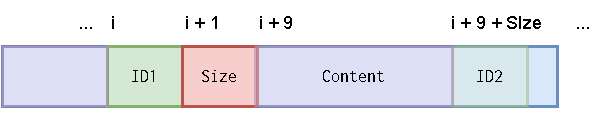
\includegraphics[width=0.5\linewidth]{figures/section.pdf}
    \caption{Memory byte representation of a \Wasm binary section, starting with a 1-byte section ID, followed by an 8-byte section size, and finally the section content.}
    \label{background:wasm:fig:section}
\end{figure}

A \wasm binary contains sections of 12 types, each with a specific semantic role and placement within the module. 
Each section is optional, where an omitted section is considered empty.
In the following text, we summarize each one of the 12 types of \wasm sections, providing their name, ID, and purpose. 
In addition, some sections are annotated as comments in the Wasm code in \autoref{WASMExample}.

\todo{Check if better with examples in each section}

\wrule{Custom Section (\texttt{00})}: Comprises two parts: the section name and arbitrary content. Primarily used for storing metadata, such as the compiler used to generate the binary. This type of section has no order constraints with other sections and is optional. Compilers usually skip this section when consuming a \Wasm binary. 

\wrule{Type Section (\texttt{01})}: Contains the function signatures for functions declared or defined within the binary. It must occur only once in a binary. It can be empty.

\wrule{Import Section (\texttt{02})}: Lists elements imported from the host, including functions, memories, globals, and tables. It must occur only once in a binary. It can be empty.

\wrule{Function Section (\texttt{03})}: Details functions defined within the binary. It essentially maps Type section entries to Code section entries. It must occur only once in a binary. It can be empty.

\wrule{Table Section (\texttt{04})}: Groups functions with identical signatures to control indirect calls. It must occur only once in a binary. It can be empty.

\wrule{Memory Section (\texttt{05})}: Specifies the number and initial size of unmanaged linear memories. It must occur only once in a binary. It can be empty. 

\wrule{Global Section (\texttt{06})}: Defines global variables as managed memory for use and sharing between functions in the \Wasm binary. It must occur only once in a binary. It can be empty.

\wrule{Export Section (\texttt{07})}: Declares elements like functions, globals, memories, and tables for host engine access. The entry point of the \Wasm binary is typically declared here. It must occur only once in a binary. It can be empty.

\wrule{Start Section (\texttt{08})}:  Designates a function to be called upon binary readiness, initializing the \Wasm program state before executing any exported functions. It must occur only once in a binary. It can be empty.

\wrule{Element Section (\texttt{09})}: Contains elements to initialize the binary tables. It must occur only once in a binary. It can be empty.

\wrule{Code Section (\texttt{10})}: Contains the body of functions defined in the Function section. Each entry consists of local variables used and a list of instructions. It must occur only once in a binary. It can be empty.

\wrule{Data Section (\texttt{11})}: Holds data for initializing unmanaged linear memory. Each entry specifies the offset and data to be placed in memoryIt must occur only once in a binary. It can be empty.

\wrule{Data Count Section (\texttt{12})}: Primarily used for validating the Data Section. If the segment count in the Data Section mismatches the Data Count, the binary is considered malformed. It must occur only once in a binary. It can be empty.


%Notice that, some sections, like the Start and Custom sections, are optional and without order constraints, offering flexibility w.r.t the \was binary layout. 
%For instance, the Custom section can store metadata, such as the compiler used to generate the binary.  

%Moreover, only a few sections have order constraints, providing additional flexibility. 


\msubsection{\Wasm's Runtime structure}
\label{background:wasm:execution}

\todo{Reorder this text according with the wrules}

The \Wasm runtime structure is described in the WebAssembly specification by enunciating 10 key components: the Store, Stack, Locals, Module Instances, Function Instances, Table Instances, Memory Instances, Global Instances, Export Instances, and Import Instances. 
These components are particularly significant in maintaining the state of a WebAssembly program during its execution. 
In the following text, we provide a brief description of each runtime component.
Notice that, the runtime structure is an abstraction that serves to validate \wasm consumers.

\wrule{Store}: The WebAssembly store represents the global state and is a collection of instances of functions, tables, memories, and globals. Each of these instances is uniquely identified by an address, which is usually represented as an i32 integer.


\wrule{Module Instances}: A module instance is a runtime representation of a loaded and initialized WebAssembly module. 
It contains the runtime representation of all the definitions within a module, including functions, tables, memories, and globals, as well as the module's exports and imports.


\wrule{Table instances}: A table instance is a vector of function elements. 
WebAssembly tables are used to support indirect function calls.
For example, it allows modeling dynamic calls of functions (through pointers) from languages such as C/C++, for which the Wasm's compiler is in charge of populating the static table of functions.


\wrule{Export Instances}: Export instances represent the functions, tables, elements, globals or memories that are exported by a module. 

\wrule{Import Instances}: Import instances represent the functions, tables, elements, globals or memories that are imported into a module from the host. 

\wrule{The Stack} holds typed values and control frames, with control frames handling block instructions, loops, and function calls.
Values inside the stack can be of the only static types allowed in Wasm 1.0, \texttt{i32} for 32 bits signed integer, \texttt{i64} for 64 bits signed integer, \texttt{f32} for 32 bits float and \texttt{f64} for 64 bits float.
Therefore, abstract types, such as classes, objects, and arrays, are not natively supported. 
Instead, during compilation, such types are transformed into primitive types and stored in the linear memory.

\wrule{Memory Instances} represent the unmanaged linear memory of a WebAssembly program, consisting of a contiguous array of bytes.
Memory instances are accessed with \texttt{i32} pointers (integer of 32 bits). 
Memory instances are usually bound in browser engines to 4Gb of size, and it is only shareable between the process that instantiates the \Wasm module and the binary itself.

\wrule{Global Instances}: A global instance is a global variable with a value and a mutability flag, indicating whether the global can be modified or is immutable.
Global variables are part of the managed data, i.e., their allocation and memory placement are managed by the host engine.
Global variables are only accessible by their declaration index, and it is not possible to dynamically address them. 


\wrule{Locals}: Locals are mutable variables that are local to a specific function invocation. As globals, locals are part of the managed data.

\begin{note}\label{managed_unmanaged}
    Along with this dissertation, as the work of Lehmann \etal \cite{usenixWasm2020}, we refer to managed and unmanaged data to differentiate between the data that is managed by the host engine and the data that is managed by the \Wasm program respectively.
\end{note}

\wrule{Function Instances}: 
A function instance groups locals and a function body.
Locals are typed variables that are local to a specific function invocation.
The function body is a sequence of instructions that are executed when the function is called.
Each instruction either reads from the stack, writes to the stack, or modifies the control flow of the function.
Recalling the example \wasm binary previously showed, 
% Functions
the local variable declarations and typed instructions that are evaluated using the stack can be appreciated between Line 7 and Line 32 in \autoref{WASMExample}. 
Each instruction reads its operands from the stack and pushes back the result. 
In the case of \autoref{WASMExample}, the result value of the main function is the calculation of the last instruction, \texttt{i32.add} at \lineref{result}. 
As the listing shows, instructions are annotated with a numeric type.


\msubsection{\Wasm's control flow}

In \Wasm, a defined function instructions are organized into blocks, with the function's starting point serving as the root block. 
Unlike traditional assembly code, control flow structures in Wasm jump between block boundaries rather than arbitrary positions within the code. 
Each block might specify the required stack state before execution and the resulting stack state after its instructions have run. 
This stack state is used to validate the binary during compilation and to ensure that the stack is in a valid state before executing the block's instructions.
Blocks in Wasm are explicit, indicating, where they start and end.
By design, each block cannot reference or execute code from outer blocks.

Control flow within a function is managed through three types of break instructions: unconditional break, conditional break, and table break. 
Importantly, each break instruction is limited to jumping to one of its enclosing blocks.
%Loops in Wasm are specialized blocks that can be restarted using a break instruction. 
Unlike standard blocks, where breaks jump to the end of the block, breaks within a loop block jump to the block's beginning, effectively restarting the loop. 
To illustrate this, \autoref{background:wasm:block} provides an example comparing a standard block and a loop block in a Wasm function.


\begin{minipage}{0.95\linewidth}
   
   \begin{minipage}{0.45\linewidth}
      \lstset{
      language=WAT,
      style=WATStyle,
      breaklines=true, 
      %stepnumber=0,
      escapeinside={(*@}{@*)},
      numbers=none,
      postbreak=\mbox{\space},
      label=BlockExample}

   \begin{lstlisting}    
block
   block
      br 1 (*@\tikzmarkMap{2}{}{8.5}{2}{2cm}@*) ; Jump instructions are annotated with the depth of the block they jump to; 
   end (*@\tikzmarkMap{7}{}{8.5}{0}{2cm}@*)
end (*@\tikzmarkMap{1}{}{8}{3}{2cm}@*)
... (*@\tikzmarkMap{9}{}{8.5}{2}{2cm}@*)
   \end{lstlisting}
   \end{minipage}\hspace{1mm}
   \begin{minipage}{0.44\linewidth}
   \lstset{
      language=WAT,
      style=WATStyle,
      breaklines=true, 
      %stepnumber=0,
      escapeinside={(*@}{@*)},
      numbers=none,
      postbreak=\mbox{\space},
      label=LoopExample}

   \begin{lstlisting}    
loop (*@\tikzmarkMap{6}{}{8.5}{2}{2cm}@*)
   ...
   br 0 (*@\tikzmarkMap{5}{}{8.5}{2}{2cm}@*) ;first-order break;
   ... 
end (*@\tikzmarkMap{3}{}{8.5}{2}{2cm}@*) ; end instructions break the block and jump to next instruction; 
... (*@\tikzmarkMap{4}{}{8.5}{-2}{2cm}@*)
   \end{lstlisting}
   \end{minipage}
   \begin{tikzpicture}[remember picture,overlay]

      %\path (2.west) edge[<-, black] (1.west);
      %\path (3.west) edge[<-,  black] (4.west);
   
      \path (1.west) edge[<-, bend right, black] (2.west);
      %\path (1.west) edge[<-, bend right, gray] (7.west);
      %\path (9.west) edge[<-, bend right, gray] (1.west);
   
      \path (4.west) edge[<-, bend right, gray] (3.west);
      \path (6.west) edge[<-, bend left, black] (5.west);
      %\path (9.east) edge[<-, bend right, black] (4.east);
      %\path (7.east) edge[<-, bend right, black] (8.east);
   
      \end{tikzpicture}
      \centering
      \hrule
      \vspace{2mm}
      \captionof{lstlisting}{Example of breaking a block and a loop in \Wasm.}
      \label{background:wasm:block}
\end{minipage}
% Example


Each break instruction includes the depth of the enclosing block as an operand. 
This depth is used to identify the target block for the break instruction. 
For example, in the left-most part of the previously discussed listing, a break instruction with a depth of 1 would jump past two enclosing blocks.
For the purposes of this dissertation, we introduce a specific term to describe a particular kind of break within loops:

\begin{definition}\label{first_order_jump}
Break instructions within loops that effectively jump to the loop's beginning are termed \emph{first-order breaks}.
\end{definition}


\msubsection{WebAssembly's Ecosystem}
\label{background:wasm:ecosystems}



\Wasm programs are designed for execution in host environments such as web browsers.
Though the execution of a \Wasm program might be considered its final lifecycle stage, the \Wasm ecosystem is far from simplistic.
It comprises multiple stakeholders and a rich array of tools that cater to various needs \cite{Avenger}.
%To the best of our knowledge, the most complete survey about Wasm tooling is presented in the Awesome Wasm  (\url{https://github.com/mbasso/awesome-wasm}) repository. 
%It is a cumulative GitHub repository which includes references to articles, papers, books, demos, compilers and engines related to \wasm.
%We have complemented our findings with selecting a subset of the tools mentioned in the Awesome Wasm repository to illustrate the \Wasm ecosystem. 
In \autoref{wasm:background:landscape} we simplify the ecosystem landscape by separating it into producers, consumers and major stakeholders categories.
In the subsequent text, we describe the \Wasm ecosystem by separating it into stakeholders categories.

\begin{figure}
    \centering
    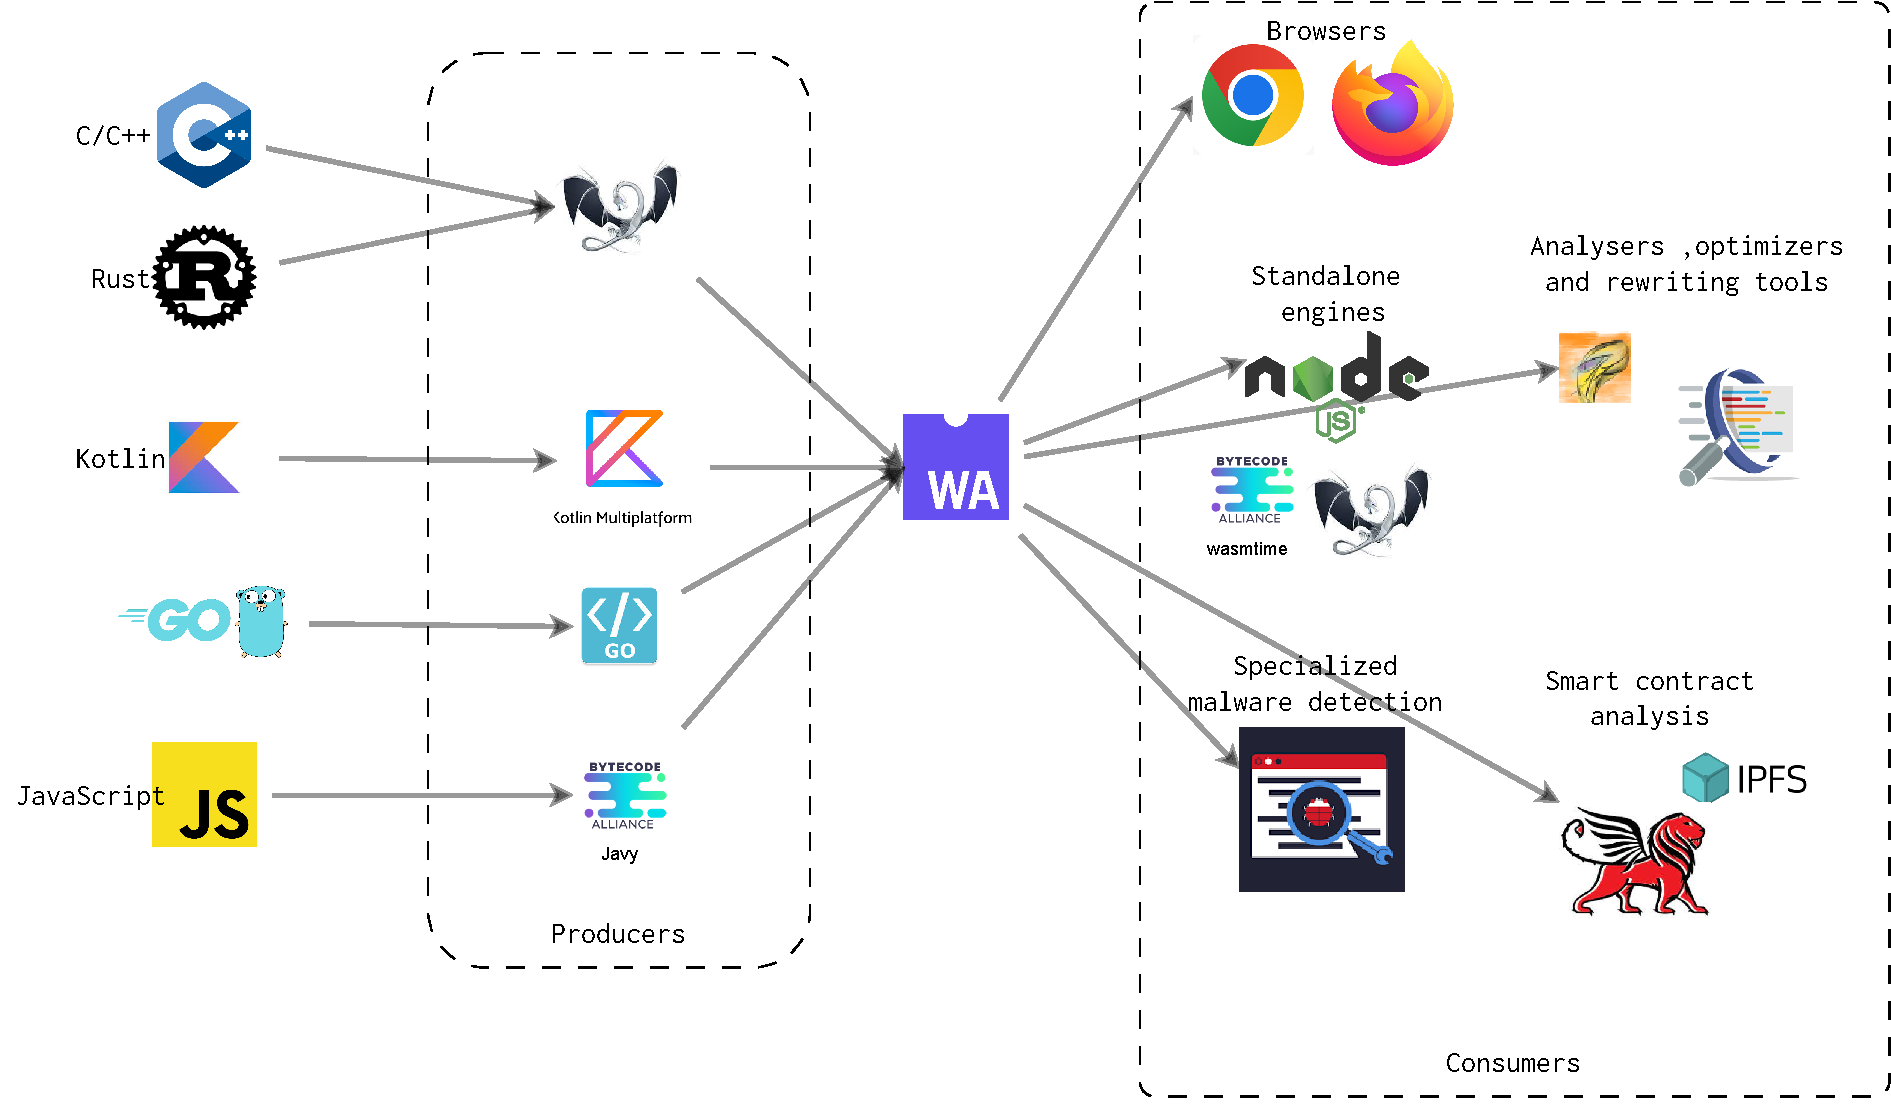
\includegraphics[width=1.0\linewidth]{figures/landscape2.pdf}
    \caption{\Wasm's ecosystem landscape separated into producers and consumers. For the sake of simplicity we do not include each tool mentioned in this chapter.}
    \label{wasm:background:landscape}
\end{figure}

\wrule{Producers}, such as compilers, transform source code into \Wasm binaries. 
For example, LLVM has offered \Wasm as a backend option since its 7.1.0 release\footnote{\url{https://github.com/llvm/llvm-project/releases/tag/llvmorg-7.1.0}}, supporting a diverse set of frontend languages like C/C++, Rust, Go, and AssemblyScript\footnote{A subset of the TypeScript language}.
In parallel developments, the KMM framework\footnote{\url{https://kotlinlang.org/docs/wasm-overview.html}} has incorporated \Wasm as a compilation target, and the Javy approach\footnote{\url{https://github.com/bytecodealliance/javy}} focuses on encapsulating JavaScript code within isolated \Wasm binaries. 
This is achieved by porting both the engine and the source code into a secure \Wasm environment. 
Blazor also enables the compilation of C# code into \Wasm binaries for browser execution\footnote{\url{https://dotnet.microsoft.com/apps/aspnet/web-apps/blazor}}.
Regardless of the source language or framework, the resulting \Wasm binary functions similar to a traditional shared library, replete with code instructions, symbols, and exported functions.
%From a security standpoint, \Wasm programs are designed without a standard library and are prohibited from direct interactions with the operating system. Instead, the host environment offers a predefined set of functions that can be imported into the \Wasm program. 
%It falls upon the producers to specify which functions from the host environment will be imported by the \Wasm application.

\wrule{Consumers} encompass tools that undertake the tasks of validating, analyzing, optimizing, transpiling to machine code, and executing \Wasm binaries, e.g. browser clients. 
In the text that follows, we dissect them into specific categories and their respective domains of application.
Notice that, while some tools are designed for a specific domain, others are more general-purpose and might encapsulate more than one task in the \Wasm ecosystem.
For example, this is the case of browsers and standalone engines, which in one way or the other perform each one of the previous tasks.


\wrule{Browser} engines like V8\cite{v8}, SpiderMonkey\cite{spidermonkey}, and Chakra\cite{chakra} are at the forefront of executing \Wasm binaries in browser clients. 
These engines leverage Just-In-Time (JIT) compilers to convert \Wasm into machine code. 
This translation is typically a straightforward one-to-one mapping, given that \Wasm is already an optimized format closely aligned with machine code, as previously discussed in \autoref{background:wasm:binary}. 
For example, V8 employs quick, rudimentary optimizations such as constant folding and dead code removal\footnote{This analysis was corroborated through discussions with the V8 development team and through empirical studies in one of our contributions\cite{CROW}}. 

\wrule{Standalone engines} \Wasm's applicability has transcended browser environments, largely due to the WebAssembly System Interface (WASI)\cite{WASI}. 
WASI aims to standardize the interaction between host environments and \Wasm modules, thereby facilitating portability of both bytecode and binaries across diverse platforms. 
It outlines a POSIX-like Application Binary Interface (ABI), which includes functionalities for filesystem access, network sockets, clocks, and random number generation, among others. 
Standalone engines such as WASM3\cite{wasm3}, wasmtime\cite{wasmtime}, WAVM\cite{WAVM} and Sledge \cite{Sledge} have emerged to support \Wasm and WASI.
Similarly, Singh and colleagues \cite{WARDuino2019} proposed a virtual machine for Wasm in Arduino based devices.


\todo{Disect them into, JIT compilers and interpreters, ending with SWAM.}
\todo{Add the verifiable standalone engine here}


\todo{Locate WasmA} \cite{WasmA}

\wrule{Static and dynamic analysis, optimization and validation:} Tools such as Wassail\cite{wassail}, Wasmati\cite{wasmati}, and Wasp\cite{Wasp} utilize a range of strategies, including information flow control, code property graphs, and concolic execution, to identify vulnerabilities taking \wasm programs as input. 
Dynamic analysis counterparts like TaintAssembly\cite{taintassembly}, Wasabi\cite{wasabi}, and Fuzzm\cite{fuzzm} serve analogous functions.
\todo{Binanryen}
\todo{\url{https://soft.vub.ac.be/Publications/2023/vub-tr-soft-23-11.pdf}, \url{https://dl.acm.org/doi/abs/10.1145/3510003.3510070?casa_token=hAlPiu9_oioAAAAA:DskwqdqM8c5-4e4W-8uU2CiENeyyOXWoi6BHytTiZUgyxojsYWXBsaS7ERFeqGNKfaYIKIN8pnQ1}}
\todo{Wafl}
\todo{Add veriwasm}
\todo{Wasmfuzzer}

\wrule{Specialized Malware Detection} In niche areas like cryptomalware detection, tools like MineSweeper\cite{Minesweeper}, MinerRay\cite{MinerRay}, and MINOS\cite{MINOS} utilize static analysis techniques. 
Conversely, dynamic analysis is the forte of tools like SEISMIC\cite{SEISMIC}, RAPID\cite{RAPID}, and OUTGuard\cite{outguard}.

\wrule{Smart Contract Analysis} In the field of smart contracts, static analysis tools like EvalHunter\cite{evalhunter}, WANA\cite{wana}, and EOSAFE\cite{eosafe} are employed to unearth vulnerabilities in \Wasm-based contracts. Dynamic analysis tools in this sphere include EOSFuzzer\cite{eosfuzzer} and wasai\cite{wasai}.


\wrule{Obfuscation, and binary rewriting tools} \cite{wasmixer} \cite{wobfuscator} \todo{WASMixer, Wobfuscator}


% Open challenges
% \msubsection{Opportunities}

While many existing tools purport to offer self-correctness evaluations and exhaustive test suites, the \Wasm ecosystem is still in its early stages. 
To emphasize this, a 2021 study by Hilbig et al.\cite{Hilbig2021AnES} found a mere 8,000 unique \Wasm binaries globally. 
This pales in comparison to mature ecosystems like JavaScript and Python, which offer 1.5 million and 1.7 million packages on npm\footnote{\url{https://www.npmjs.com/}} and PyPI\footnote{\url{https://pypi.org/}}, respectively.
This limited pool of \Wasm binaries presents a unique challenge for machine learning-based analysis tools, which require large datasets for effective training. 
This issue is explicitly addressed in one of the contributions of this dissertation\cite{EVASION}.
Additionally, the scarcity of \Wasm programs exacerbates the problem of software monoculture, increasing the likelihood of consuming a compromised \Wasm program\cite{YourCitationHere}.
Besides, the current size of the \Wasm ecosystem offers a small testing environment for evaluating the capabilities of consumer tools.
This dissertation aims to address these issues by introducing a comprehensive suite of tools. 
These tools are crafted to not only bolster the security of \Wasm programs through Software Diversification but also to intensify the testing rigor for both producers and consumers in the ecosystem.


\msubsection{WebAssembly's Security}

\todo{Check the attack primitives defined by Lehmann.}
\todo{Extend with more cases !}

As we described, \wasm\ is deterministic and well-typed, follows a structured control flow and explicitly separates its linear memory model, global variables and the execution stack. This design is robust \cite{WebAssemblySecurity} and makes it easy for compilers and engines to sandbox the execution of Wasm  binaries. Following the specification of Wasm  for typing, memory, virtual stack and function calling,
host environments should provide protection against data corruption, code injection, and return-oriented programming (ROP).

However, implementations in both browsers and standalone runtimes~\cite{Narayan2021Swivel} are vulnerable.
Genkin \etal demonstrated that Wasm  could be used to exfiltrate data using cache timing-side channels \cite{Genkin2018DrivebyKC}.
Moreover, binaries itself can be vulnerable. The work of Lehmann \etal ~\cite{usenixWasm2020} proved that C/C++ source code vulnerabilities can propagate to Wasm  such as overwriting constant data or manipulating the heap by overflowing the stack. Even though these vulnerabilities need a specific standard library implementation to be exploited, they make a call for better defenses for \wasm. 
Recently, Stiévenart and colleagues demonstrate that C/C++ source code vulnerabilities can be ported to Wasm \cite{DeRoover2022}.
% Current proposals
Several proposals for extending \wasm\ in the current roadmap could address some existing vulnerabilities. For example, having multiple memories\footnote{\url{https://github.com/WebAssembly/multi-memory/blob/main/proposals/multi-memory/Overview.md}} could incorporate more than one memory, stack and global spaces, shrinking the attack surface. However, the implementation, adoption and settlement of the proposals are far from being a reality in all browser vendors\footnote{\url{https://webassembly.org/roadmap/}}. 
% In fact, according to the work of Hilbig \etal \cite{Hilbig2021AnES}, the artificial variants created with one of our works contribute to the half of executable and available \wasm\ binaries in the wild.
